%versi 2 (8-10-2016)
\chapter{Landasan Teori}
\label{chap:teori}

\lstdefinelanguage{JavaScript}{
  keywords={new, true, false, function, return, null, catch, switch, var, if, while, do, else, const, this,Math},
  keywordstyle=\color{blue}\bfseries,
  ndkeywords={moveTo,lineTo,arc,random,floor},
  ndkeywordstyle=\color{purple}\bfseries,
  identifierstyle=\color{black},
  sensitive=false,
  comment=[l]{//},
  morecomment=[s]{/*}{*/},
  commentstyle=\itshape\color{green},
  stringstyle=\color{red},
  morestring=[b]',
  morestring=[b]",
  captionpos=b,
}

\lstset{
   language=JavaScript,
   backgroundcolor=\color{white},
   extendedchars=true,
   basicstyle=\fontfamily{fvm}\selectfont\small, 
   showstringspaces=false,
   showspaces=false,
   numbers=left,
   numberstyle=\footnotesize,
   numbersep=5pt,
   tabsize=4,
   breaklines=true,
   showtabs=false,
   captionpos=b,
   frame=leftline,
   stepnumber=1,
   literate={-}{-}1{-\,-}{--}1
}

\section{\textit{Snake}}
\label{sec:snake}
\textit{Snake} merupakan permainan mengendalikan ular untuk mendapatkan makanan yang terdapat pada labirin. Dalam permainan ini, pemain mengendalikan ular untuk mendapatkan makanan sebanyak-banyaknya. Setiap ular memakan makanan, maka skor akan bertambah 1 poin dan tubuh ular akan bertambah panjang. Biasanya makanan hanya ada 1 saja pada sebuah labirin. Ketika makanan itu sudah termakan oleh ular, makanan tersebut akan ditempatkan secara acak. Ular dapat bergerak ke atas, bawah, kiri, dan kanan. Namun pada permainan \textit{Snake} yang akan dibuat sekarang, ular dapat bergerak ke segala arah seperti ilustrasi pada Gambar~\ref{fig:ularSegalaArah}. Permainan akan berakhir jika ular menabrak dinding yang terdapat pada labirin atau ular tersebut menabrak tubuhnya sendiri. \\

\begin{figure}[H]
	\centering  
	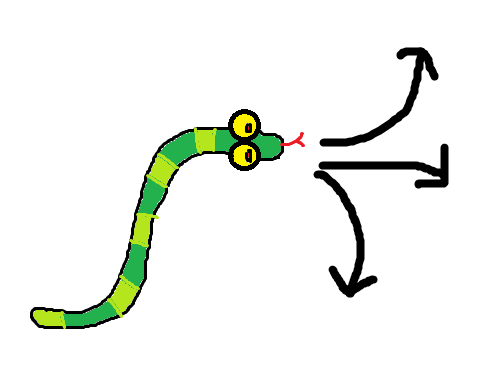
\includegraphics[scale=0.4]{ular-segala-arah}  
	\caption[Pergerakan ular ke segala arah]{Pergerakan ular ke segala arah} 
	\label{fig:ularSegalaArah} 
\end{figure} 

Permainan \textit{Snake} ini dapat dimainkan secara \textit{singleplayer} atau \textit{multiplayer}. \textit{Singleplayer game} adalah permainan yang dapat dimainkan oleh 1 pemain. \textit{Multiplayer game} adalah permainan yang dapat dimainkan oleh beberapa pemain. Pada umumnya, permainan \textit{Snake} dimainkan secara \textit{singleplayer}. Contoh \textit{singleplayer game Snake} adalah \textit{Snake} pada telepon genggam \textit{Nokia} yang dapat dilihat pada Gambar~\ref{fig:nokiaSnake}\footnote{https://en.wikipedia.org/wiki/Snake\_(video\_game\_genre)} dan contoh \textit{multiplayer game Snake} adalah \textit{Slither.io} yang dapat dilihat Gambar~\ref{fig:slither}\footnote{https://play.google.com/store/apps/details?id=air.com.hypah.io.slither}. \textit{Snake} dapat dimainkan menggunakan \textit{smartphone} dan \textit{web browser}.  

\begin{figure}[H]
	\centering  
	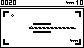
\includegraphics[scale=2]{nokiaSnake}  
	\caption[Permainan Snake pada telepon genggam \textit{Nokia}]{Permainan Snake pada telepon genggam \textit{Nokia}} 
	\label{fig:nokiaSnake} 
\end{figure} 

\begin{figure}[H]
	\centering  
	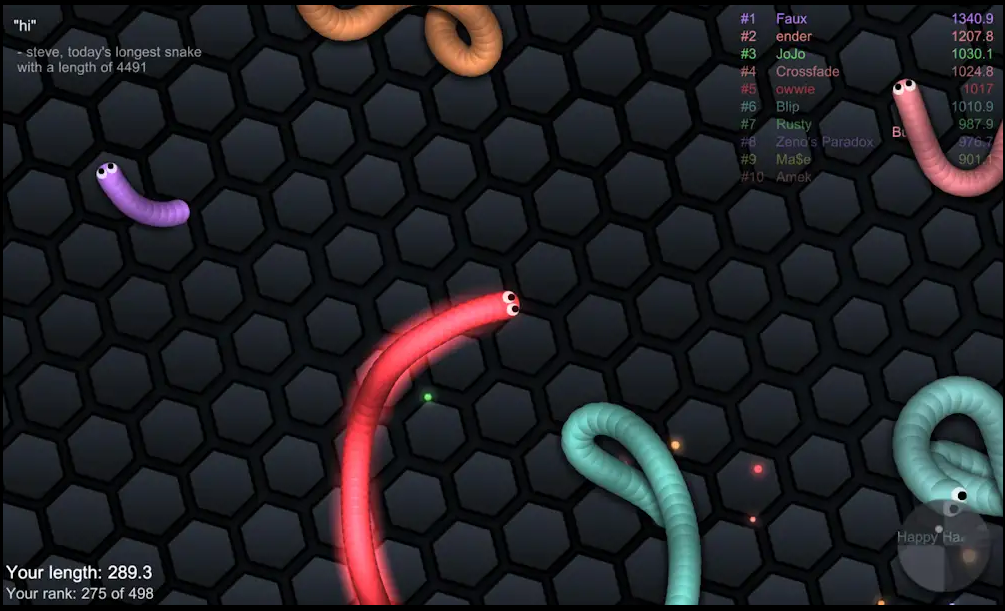
\includegraphics[scale=0.3]{slither}  
	\caption[Permainan \textit{Slither.io} pada \textit{Android}]{Permainan \textit{Slither.io} pada \textit{Android}} 
	\label{fig:slither} 
\end{figure} 

\section{HTML5 \textit{Canvas}}
\label{sec:HTML5Canvas}
HTML5 Canvas adalah sebuah daerah \textit{bitmap} yang dapat dimanipulasi oleh \textit{Javascript}. Pada daerah \textit{bitmap} tersebut, \textit{pixel-pixel} akan di\textit{render} oleh canvas. Setiap \textit{frame}, HTML5 Canvas akan menggambar pada area \textit{bitmap} tersebut menggunakan \textit{Canvas} API(\textit{Application Programming Interface}) yang dipanggil pada \textit{Javascript}. API dari HTML5 Canvas yang umum adalah 2D \textit{Context}. Dengan adanya 2D \textit{Context}, \textit{programmer} dapat membuat bentuk 2D, menampilkan gambar, \textit{render} tulisan, memberi warna, membuat garis dan kurva, dan manipulasi \textit{pixel}. HTML5 Canvas tidak hanya digunakan untuk menggambar dan menampilkan gambar serta tulisan. HTML5 Canvas dapat digunakan untuk membuat animasi, aplikasi pada \textit{web} dan permainan. 

Untuk menambahkan \textit{canvas} pada halaman HTML, diperlukan \textit{tag} <canvas>. Di bawah ini adalah potongan kode untuk menambahkan \textit{canvas} pada halaman HTML. 

\begin{lstlisting}[language=HTML, caption=Menambahkan \textit{canvas}]
	<canvas id='canvas' width='500' height='300'>
		Your browser does not support HTML5 Canvas.
	</canvas>
	
\end{lstlisting}


Berikut adalah penjelsan atribut yang ada pada \textit{canvas} berdasarkan potongan kode di atas : 
\begin{itemize}
	\item id
\end{itemize}


\section{\textit{\textit{Javascript}}}
\label{sec:Javascript}
\textit{Javascript} adalah bahasa pemrograman yang ringan, \textit{interpreted} dan berorientasi objek yang digunakan pada halaman \textit{web}. \textit{Javascript} dapat membuat objek dengan menambahkan \textit{method} dan atributnya sama seperti bahasa pemrograman C++ dan \textit{Java}. Setelah objek diinisialisasi, maka objek tersebut dapat dijadikan \textit{blueprint} untuk membuat objek lain yang mirip\footnote{https://developer.mozilla.org/en-US/docs/Web/JavaScript/About\_JavaScript}. \textit{Javascript} dapat digunakan untuk mengimplementasi hal yang kompleks pada halaman web. Contohnya adalah menamplikan peta yang interaktif dan membuat animasi 2D/3D. Selain \textit{Javascript}, HTML(\textit{HyperText Markup Language}) dan CSS(\textit{Cascading Style Sheet}) merupakan bagian/komponen penting dalam pembuatan halaman \textit{web}\footnote{https://developer.mozilla.org/en-US/docs/Learn/JavaScript/First\_steps/What\_is\_JavaScript}.\\

Untuk menambahkan Javascript pada sebuah halaman web yang dibuat, gunakan tag <script>. Ada 2 cara untuk menambahkan Javascript yaitu menambahkan langsung di halaman web tersebut(Internal Javascript) dan menambahkan file Javascript terpisah(External Javascript).

\subsection{Variabel}
Variabel adalah sebuah wadah untuk menyimpan nilai/\textit{value}. Untuk mendeklarasi variable pada \textit{Javascript}, digunakan \textit{keyword 'var'}. Variabel pada Javascript tidak perlu menuliskan tipe datanya ketika mendeklarasikan variabel. Di bawah ini adalah potongan kode untuk mendeklarasikan variabel.\footnote{https://developer.mozilla.org/en-US/docs/Web/JavaScript/Guide/Grammar\_and\_types}

\begin{lstlisting}[language=Javascript, caption=Deklarasi variabel]
	var myVariable;
	
\end{lstlisting}

Nilai variabel pada potongan kode di atas adalah \textit{undifined} karena variabel tersebut tidak diberi nilai/value. Di bawah ini adalah potongan kode untuk mengisi nilai pada variabel. 

\begin{lstlisting}[language=Javascript, caption=Mengisi nilai sebuah variabel]
	myVariable = 3;	
	
\end{lstlisting}

Variabel dapat menyimpan beberapa tipe data diantaranya adalah\footnote{https://developer.mozilla.org/en-US/docs/Learn/Getting\_started\_with\_the\_web/JavaScript\_basics} :
\begin{itemize}
	\item \textit{String} : nilai yang berupa teks atau sekumpulan huruf.
	\item \textit{Number} : nilai yang berupa angka.
	\item \textit{Boolean} : nilai \textit{true/false}.
	\item \textit{Array} : struktur untuk menyimpan lebih dari 1 nilai dalam sebuah \textit{reference}
	\item \textit{Object} : semua yang ada pada Javascript termasuk objek pada HTML.
\end{itemize}

\subsection{\textit{Constant}}
\textit{Constant} adalah sebuah variabel \textit{read-only}, artinya nilai pada \textit{constant} tidak dapat diubah. Untuk mendeklarasikan \textit{constant}, digunakan \textit{keyword 'const'}. Di bawah ini adalah potongan kode untuk mendeklarasi \textit{constant}.

\begin{lstlisting}[language=Javascript, caption=Deklarasi \textit{constant}]
	const myConst = 1;
	
\end{lstlisting}

\subsection{\textit{Function}}
\textit{Function} adalah sekumpulan perintah/\textit{statements} untuk menjalankan suatu tugas atau menghitung nilai. Untuk membuat \textit{function}, digunakan \textit{keyword 'function'}, kemudian diikuti dengan nama \textit{function} tersebut, parameter yang dituliskan di dalam kurung, dan \textit{statement}/perintah \textit{Javascript} yang ditulis di dalam kurung kurawal. Parameter pada \textit{function} bisa lebih dari 1 yang penulisanya dipisahkan oleh tanda koma (,). \textit{Function} bisa memiliki parameter atau tidak. Di bawah ini adalah potongan kode untuk membuat \textit{function} penjumlahan 2 buah bilangan.

\begin{lstlisting}[language=Javascript, caption=\textit{Function} penjumlahan 2 buah bilangan]
	function penjumlahan(angka1,angka2){
		var hasil = angka1+angka2;
		return hasil;
	}
	
\end{lstlisting}

Setelah membuat \textit{function}, \textit{function} tersebut tidak langsung dieksekusi. Membuat \textit{function} hanya memberi nama \textit{function} tersebut dan mendeskripsikan apa yang akan dilakukan oleh \textit{function} tersebut apabila dipanggil. Dengan memanggil \textit{function}, maka \textit{function} akan dieksekusi\footnote{https://developer.mozilla.org/en-US/docs/Web/JavaScript/Guide/Functions}. Di bawah ini adalah potongan kode untuk memanggil \textit{function} dengan nama penjumlahan.

\begin{lstlisting}[language=Javascript, caption=Memanggil \textit{function} penjumlahan]
	penjumlahan(10,5);
	
\end{lstlisting}

\subsection{Menggambar pada \textit{Canvas}}
Sesudah menuliskan \textit{tag} <canvas> pada HTML, canvas tidak bisa langsung digambar. Karena itu perlu ditambahkan \textit{drawing context} pada \textit{Javascript}. Di bawah ini adalah potongan kode untuk menambahkan \textit{drawing context}.

\begin{lstlisting}[language=Javascript, caption=Menambahkan \textit{drawing context canvas}]
	var myCanvas = document.getElementById('canvas');
	var context = myCanvas.getContext('2d');
\end{lstlisting}

Berdasarkan potongan kode di atas, variabel myCanvas menyimpan objek dengan id = 'canvas'. Id ini mengacu ke objek \textit{canvas} pada HTML yang memilki id bernama canvas. Variabel myCanvas sekarang sudah menyimpan objek \textit{canvas}. Kemudian variabel context menyimpan \textit{drawing context} 2D. Sesudah itu, \textit{canvas} tersebut dapat digambar dengan bentuk 2D, garis, kurva, membuat tulisan, dan menambahkan gambar. Selain untuk menggambar, bentuk-bentuk tersebut dapat diberi warna sesuai dengan keinginan.\\

Untuk menggambar bentuk 2D atau garis, diperlukan koordinat x dan y. Koordinat tersebut akan menempatkan gambar tersebut pada \textit{canvas}. Posisi awal/\textit{origin} pada \textit{canvas} adalah (0,0) yang terletak di ujung kiri atas \textit{canvas}. Gambar~\ref{fig:grid}\footnote{https://developer.mozilla.org/en-US/docs/Web/API/Canvas\_API/Tutorial/Drawing\_shapes} adalah penempatan kotak biru pada \textit{canvas} terhadap \textit{origin}.

\begin{figure}[H]
	\centering  
	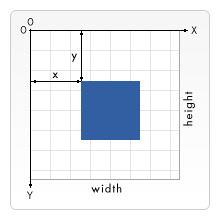
\includegraphics[scale=0.5]{grid}
	\caption[Posisi kotak biru pada \textit{canvas} terhadap \textit{origin}]{Posisi kotak biru pada \textit{canvas} terhadap \textit{origin}}
	\label{fig:grid} 
\end{figure} 

Pada di atas, titik ujung kiri kotak biru tersebut berjarak x \textit{pixel} dari kiri dan berjarak y \textit{pixel} dari atas. 

\subsubsection{Menggambar Persegi Panjang}
Ada 3 cara untuk menggambar persegi panjang:

\begin{itemize}
	\item \textit{fillRect(x,y,width,height)} : menggambar persegi panjang serta mengisi bagian tengah persegi panjang.
	\item \textit{strokeRect(x,y,width,height)} : menggambar \textit{outline} yang berbentuk persegi panjang.
	\item \textit{clearRect(x,y,width,height)} : menghapus daerah yang ditentukan pada \textit{canvas}. Daerah yang dihapus berbentuk persegi panjang.
	\item \textit{rect(x,y,width,height)} : menambah \textit{path} berbentuk persegi panjang.
\end{itemize}

Fungsi tersebut memiliki parameter yang sama. Parameter x dan y untuk menentukan posisi pada canvas dari titik ujung kiri atas persegi panjang. \textit{Width} adalah lebar dari persegi panjang dan \textit{height} adalah tinggi dari persegi panjang.

\subsubsection{Menggambar \textit{Path}}
\textit{Path} adalah sekumpulan titik yang dihubungkan oleh segmen garis. \textit{Path} dapat membentuk kurva dan membuat bentuk 2D lainnya seperti segitiga, trapesium, belah ketupat dan lain-lain. Langkah-langkah untuk membuat bentuk menggunakan path adalah sebegai berikut : 

\begin{enumerate}
	\item Buat \textit{path}.
	\item Tuliskan perintah untuk menggambar pada \textit{path} tersebut.
	\item Sesudah \textit{path} tersebut sudah dibuat, \textit{path} tersebut dapat di\textit{render} menggunakan \textit{stroke} atau \textit{fill}.
\end{enumerate}

Langkah pertama untuk membuat \textit{path} baru adalah dengan menggunakan fungsi \textit{beginPath()}. Setelah itu, perintah-perintah untuk menggambar dapat digunakan untuk membuat bentuk-bentuk yang diinginkan. Apabila sudah selesai menggambar, gunakan fungsi \textit{stroke()} untuk menggambar outline dari \textit{path} tersebut atau \textit{fill()} untuk mengisi area path tersebut. Setelah itu, gunakan fungsi \textit{closePath()} untuk menutup bentuk tersebut dengan cara menggambar garis lurus dari posisi titik terakhir ke titik awal. Fungsi lainnya yang menjadi bagian dari membuat \textit{path} adalah fungsi \textit{moveTo()}. Fungsi ini diibaratkan seperti mengangkat sebuah pensil dari sebuah titik pada kertas kemudian menempatkanya pada titik yang diinginkan. Di bawah ini adalah fungsi \textit{moveTo()}.

\begin{lstlisting}[language=Javascript, caption=Fungsi \textit{moveTo()}]
	moveTo(x,y);
\end{lstlisting}

Fungsi \textit{moveTo()} memiliki 2 parameter yaitu x dan y yang merupakan posisi titik pada \textit{canvas}. Ketika canvas sudah diinisialsasi dan fungsi \textit{beginPath()} sudah dipanggil, fungsi \textit{moveTo()} berguna sebagai penempatan titik awal untuk menggambar. Fungsi \textit{lineTo()} digunakan untuk menggambar sebuah garis. Di bawah ini adalah fungsi \textit{lineTo()}.

\begin{lstlisting}[language=Javascript, caption=Fungsi \textit{lineTo()}]
	lineTo(x,y);
\end{lstlisting}

Fungsi \textit{lineTo()} memiliki 2 parameter yaitu x dan y yang merupakan titik akhir dari garis. Garis akan digambar mulai dari posisi titik awal sampai ke posisi titik akhir garis. Titik awal ini bergantung pada titik akhir dari \textit{path} sebelumya. Titik awal dapat diubah dengan menggunakan fungsi \textit{moveTo()}.

Fungsi \textit{arc()} digunakan untuk menggambar lingkaran atau busur. Di bawah ini adalah fungsi arc().

\begin{lstlisting}[language=Javascript, caption=Fungsi \textit{arc()}]
	arc(x,y,radius,startAngle,endAngle,anticlockwise);
\end{lstlisting}

Parameter x dan y adalah posisi titik tengah busur pada canvas. Radius adalah besar jari-jari busur. StartAngle dan endAngle adalah titik awal dan titik akhir busur dalam satuan radian yang diukur dari sumbu x. Anticlockwise adalah parameter yang bernilai boolean, apabila bernilai true, maka busur akan digambar berlawanan arah jarum jam dan jika bernilai false, busur akan digambar searah jarum jam. Karena fungsi arc() menerima input sudut dalam radian, maka perlu dilakukan konversi dari satuan derajat menjadi radian terlebih dahulu. Rumusnya adalah sebagai berikut :

\begin{displaymath}
	radian = (Math.PI / 180) * besar sudut
\end{displaymath}	

\textit{B\'ezier curve} merupakan tipe \textit{path} yang digunakan untuk membuat kurva. \textit{B\'ezier curve} ada 2 jenis yaitu \textit{cubic} dan \textit{quadratic}. Perbedaanya adalah \textit{quadratic B\'ezier curve} memiliki sebuah \textit{control point}, sedangkan \textit{cubic B\'ezier curve} memiliki 2 buah \textit{control point}. Pada Gambar~\ref{fig:bezier}\footnote{https://developer.mozilla.org/en-US/docs/Web/API/Canvas\_API/Tutorial/Drawing\_shapes} menunjukkan perbedaan antara \textit{quadratic B\'ezier curve} dan \textit{cubic B\'ezier curve}. Titik merah pada gambar merupakan \textit{control point} dari \textit{B\'ezier curve}.

\begin{figure}[H]
	\centering  
	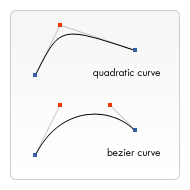
\includegraphics[scale=1]{bezier}
	\caption[Perbedaan \textit{quadratic B\'ezier curve} dan \textit{cubic B\'ezier curve}]{Perbedaan \textit{quadratic B\'ezier curve} dan \textit{cubic B\'ezier curve}}
	\label{fig:bezier} 
\end{figure} 

Berikut adalah fungsi \textit{quadratic} dan \textit{cubic B\'ezier curve} :
\begin{itemize}
	\item \textit{quadraticCurveTo(cp1,cp2,x,y)} : menggambar \textit{quadratic B\'ezier curve} dari posisi pensil sekarang ke titik akhir yaitu x dan y, dengan titik control point yaitu cp1 dan cp2.
	\item bezierCurveTo(cp1x,cp1y,cp2x,cp2y,x,y) : menggambar \textit{cubic B\'ezier curve} dari posisi pensil sekarang ke titik akhir yaitu x dan y, dengan 2 titik control point yaitu (cp1x,cp1y) dan (cp2x,cp2y).
\end{itemize}

\subsection{\textit{Object Oriented Programming Javascript}}
OOP (\textit{Object Oriented Programming}) adalah sebuah paradigma \textit{programming} yang menggunakan abstraksi untuk membuat objek-objek yang ada pada dunia nyata. Bahasa pemrograman seperti \textit{Java}, C++, \textit{Ruby, Phyton}, PHP, dan \textit{Objective-C} sudah mendukung OOP. Dalam OOP, setiap objek dapat menerima pesan, memproses data dan mengirim pesan ke objek lain. Program yang menggunakan konsep OOP ini mudah untuk dimengerti dan lebih mudah untuk dikembangkan oleh \textit{programmer}\footnote{https://developer.mozilla.org/ms/docs/Web/JavaScript/Introduction\_to\_Object-Oriented\_JavaScript}. \\

Ide umum pada OOP adalah menggunakan objek untuk memodelkan benda-benda yang ada pada dunia nyata. Objek tersebut kemudian direpresentasi pada program yang dibuat. Objek-objek dapat berisi data, fungsionalitas dan \textit{behaviour} yang merepresentasikan informasi tentang objek tersebut dan tugas objek\footnote{https://developer.mozilla.org/en-US/docs/Learn/JavaScript/Objects/Object-oriented\_JS}. Contohnya, bila ingin membuat objek sebuah mobil. Mobil memiliki beberapa informasi diantaranya adalah merk mobil, berat mobil, warna mobil dan tahun produksi. Informasi tersebut dapat disebut sebagai properti dari objek. Mobil dapat bergerak maju, berbelok ke kanan, berbelok ke kiri, bergerak mundur dan berhenti. Hal-hal yang dapat dilakukan oleh objek disebut sebagai method dari objek. 

\subsubsection{Kelas}
Javascript tidak memiliki statement 'class' yang dapat digunakan pada bahasa pemrograman C++ atau \textit{Java}. Untuk membuat kelas, Javascript menggunakan \textit{function} sebagai konstruktor untuk kelas. Karena itu, membuat kelas sama dengan membuat \textit{function} pada Javascript. Di bawah ini adalah potongan kode untuk membuat kelas bernama Mobil.

\begin{lstlisting}[language=Javascript, caption=Membuat kelas Mobil]
	function Mobil(){
	
	}
	
\end{lstlisting}

\subsubsection{Objek}
Untuk membuat instansi baru dari objek, gunakan statement 'new' yang nantinya akan disimpan pada variabel. Di bawah ini adalah potongan kode untuk membuat \textit{instance}.

\begin{lstlisting}[language=Javascript, caption=Membuat \textit{instance} mobil]
	var mobil1 = new Mobil();
\end{lstlisting}

\subsubsection{Konstruktor}
Konstruktor adalah method yang ada pada kelas. Konstruktor akan dipanggil ketika pertama kali inisialisasi atau saat instansi baru dari objek dibuat. \textit{Function} pada Javascript berfungsi sebagai konstruktor sehingga tidak perlu membuat method konstruktor lagi. Semua aksi yang terdapat pada kelas akan dieksekusi pada saat instansiasi.

\subsubsection{Properti/Atribut}
Properti adalah variabel yang terdapat pada kelas. Properti ditulis pada konstruktor kelas sehingga setiap properti pada kelas akan dibuat ketika membuat instansi baru. Untuk membuat properti, gunakan statement 'this'. Cara ini mirip dengan bahasa pemrograman Java ketika membuat sebuah properti pada objek. Syntax untuk mengakses properti di luar kelas adalah : namaInstansi.properti. Di bawah ini adalah potongan kode untuk mendefinisikan properti pada kelas Mobil pada saat instansiasi.

\begin{lstlisting}[language=Javascript, caption=Mendefinisikan properti pada kelas Mobil]
	function Mobil(merkMobil,beratMobil,warnaMobil,tahunProduksi){
		this.merkMobil = merkMobil;
		this.beratMobil = beratMobil; //satuan dalam kg
		this.warnaMobil = warnaMobil;
		this.tahunProduksi = tahunProduksi;
	}
	
	var mobil1 = new Mobil('Toyota',1000,'Hitam',2010);
	
\end{lstlisting}

\subsubsection{Method}
Method adalah hal yang dapat dilakukan oleh sebuah objek. Untuk membuat method, tuliskan nama method terlebih dahulu kemudian \textit{assign} fungsi pada nama method tersebut. Untuk memanggil method sebuah objek, tuliskan nama objek/kelas terlebih dahulu, kemudian tuliskan nama method sesuai dengan yang sudah dibuat beserta tanda kurung. Tanda kurung berisi parameter. Di bawah ini adalah potongan kode untuk membuat dan memanggil method bergerakMaju() pada kelas Mobil.

\begin{lstlisting}[language=Javascript, caption=Membuat dan memanggil method bergerakMaju()]
	function Mobil(merkMobil,beratMobil,warnaMobil,tahunProduksi){
		this.merkMobil = merkMobil;
		this.beratMobil = beratMobil; //satuan dalam kg
		this.warnaMobil = warnaMobil;
		this.tahunProduksi = tahunProduksi;
		
		this.bergerakMaju = function(){
			//kode agar mobil bergerak maju
		}
	}
	
	var mobil1 = new Mobil('Toyota',1000,'Hitam',2010);
	mobil1.bergerakMaju(); //memanggil fungsi untuk bergerak maju
	
\end{lstlisting}

\subsection{\textit{Events}}
Events adalah kejadian/peristiwa yang terjadi pada sistem yang diprogram. Sistem akan memberitahu apabila kejadian tersebut sudah terjadi dan akan melakukan suatu aksi ketika kejadian sudah terjadi. Misalnya, di bandara ketika landasan pacu sudah bersih untuk pesawat lepas landas, sinyal akan dikomunikasikan kepada pilot bahwa pesawat sudah boleh untuk lepas landas. Dalam web, events ditembakan di dalam \textit{browser window} dan dikaitkan pada objek yang spesifik seperti sekumpulan elemen, dokumen HTML yang dimuat atau keseluruhan \textit{browser window}. Ada beberapa events yang dapat terjadi diantaranya adalah : 

\begin{itemize}
	\item Pengguna mengklik sebuah element atau mengarahkan kursor ke sebuah elemen.
	\item Pengguna menekan sebuah tombol pada keyboard.
	\item Pengguna mengatur besar dan menutup browser window.
	\item Halaman web selesai dimuat.
	\item Form sedang disubmit.
	\item Video sedang dimainkan, dijeda, atau selesai.
	\item Ketika error terjadi.
\end{itemize}

Setiap events memiliki event handler, yang berisikan sekumpulan kode yang akan dijalankan ketika event sudah terjadi. Event handler juga sering disebut sebagai event listener. Listener menunggu event yang terjadi dan handler adalah kode yang dijalankan ketika listener mendapatkan event/ketika event terjadi. Untuk memperjelas bagaimana cara menggunakan event, di bawah ini terdapat contoh kode untuk menambahkan event pada button/tombol.

\begin{lstlisting}[language=Javascript,{alsolanguage=HTML}, caption=Menambahkan event pada button]
	<html>
		<title>Event pada tombol</title>
		<body>
			<button id='tombol'>Change color</button>
		</body>
	</html>
	
	<script>
		var btn = document.getElementById('tombol');

		function random(number) {
  			return Math.floor(Math.random()*(number+1));
		}

		btn.onclick = function() {
  			var rndCol = 'rgb(' + random(255) + ',' + random(255) + ',' + random(255) + ')';
  			document.body.style.backgroundColor = rndCol;
		}
	</script>
	
\end{lstlisting}

Berdasarkan kode di atas, objek button dengan id='tombol' disimpan di dalam variabel bernama 'btn'. Ada fungsi bernama 'random' untuk mengembalikan sebuah nilai acak. Setelah itu ada event handler. Event handler property yang digunakan adalah onclick. Event handler property onclick mengecek apakah objek(dalam kasus ini objeknya adalah button) sudah ditekan/diklik. Bila tombol sudsh diklik, maka akan mengeksekusi fungsi untuk mengubah warna background. Warna RGB tersebut digenerate secara acak menggunakan fungsi random yang sudah dibuat sebelumnya. Tidak hanya event handler property onclick saja yang dapat digunakan pada halaman web. Berikut ini adalah beberapa event handler property lainnya:

\begin{itemize}
	\item onfocus dan onblur : event akan terjadi apabila sebuah objek difokuskan/tidak. Biasanya digunakan untuk menampilkan informasi tentang bagaimana cara mengisi form ketika difokuskan atau menampilkan pesan error ketika form tersebut diisi dengan nilai yang salah/tidak valid.
	\item ondblclick : event akan terjadi ketika objek diklik 2 kali/double click.
	\item window.keypress, window.onkeydown, window.onkeyup : event akan terjadi apabila sebuah tombol pada keyboard ditekan. Keypress adalah event ketika tombol ditekan kemudian dilepas. Keydown adalah event ketika tombol ditekan dan keyup adalah event ketika tombol dala m keadaan tidak ditekan. Untuk ketiga event ini, event tersebut harus diregister pada object window yang merepresentasikan browser window.
	\item onmouseover dan onmouseout : event akan terjadi ketika posisi kursor mouse berada luar objek lalu ditempatkan di atas objek dan ketika posisi kursor mouse berada di atas objek lalu keluar dari objek. 
\end{itemize}

Beberapa event handler property tersebut sangat umum dan tersedia di manapun, sedangkan beberapa event handler property lainnya sangat spesifik dan hanya digunakan untuk elemen tertentu, contohnya adalah menggunakan onplay untuk elemen tertentu yaitu <video>.

Mekanisme event terbaru dalam spesifikasi DOM(Document Object Model) level 2 Events yang memberikan browser sebuah fungsi baru yaitu addEventListener(). Fungsi ini mirip seperti event handler property namun memiliki sintaks yang berbeda. Di bawah ini adalah potongan kode untuk menggunakan fungsi addEventListener().

\begin{lstlisting}[language=Javascript, caption=Menggunakan fungsi addEventListener()]

	var btn = document.getElementById('tombol');

	function bgChange() {
  		var rndCol = 'rgb(' + random(255) + ',' + random(255) + ',' + random(255) + ')';
  		document.body.style.backgroundColor = rndCol;
	}   

	btn.addEventListener('click', bgChange);
	
\end{lstlisting}

Pada fungsi addEventListener(), ada 2 buah parameter yaitu event yang ingin digunakan(dalam potongan kode di atas menggunakan event click) dan kode sebagai handler yang ingin dijalankan ketika event tersebut terjadi. Selain cara di atas, dapat juga menuliskan semua kode di dalam fungsi addEventListener() seperti potongan kode di bawah ini.

\begin{lstlisting}[language=Javascript, caption=Menuliskan kode di dalam fungsi addEventListener()]

	btn.addEventListener('click', function() {
  		var rndCol = 'rgb(' + random(255) + ',' + random(255) + ',' + random(255) + ')';
  		document.body.style.backgroundColor = rndCol;
	});
	
\end{lstlisting}


\subsection{Membuat Animasi}
Ketika menggambar sebuah bentuk pada canvas, bentuk tersebut tidak berpindah tempat. Agar bentuk dapat bergerak, bentuk tersebut harus digambar ulang dan semua yang sudah digambar sebelumnya. Langkah-langkah untuk membuat animasi adalah sebagai berikut :

\begin{enumerate}
	\item Membersihkan canvas : hilangkan semua bentuk-bentuk yang sudah tergambar di canvas. Untuk menghapus keseluruhan canvas, gunakan fungsi clearRect().
	\item Menyimpan state canvas : ketika mengubah atribut(seperti style) yang mempengaruhi state canvas dan ingin original state tersebut digunakan kembali, state tersebut harus disimpan. 
	\item Gambar bentuk : gambar bentuk yang ingin dianimasikan.
	\item Mengembalikan state canvas : jika state sudah disimpan, kembalikan state tersebut sebelum menggambar di frame yang baru.
\end{enumerate}

Bentuk yang digambar pada canvas dapat menggunakan method/fungsi yang dimiliki oleh canvas atau dengan membuat fungsi sendiri. Hasil yang ada pada canvas akan muncul setelah script selesai mengeksekusi. Jadi dibutuhkan cara untuk mengeksekusi fungsi untuk menggambar dalam waktu tertentu. Ada 3 fungsi yang dapat digunakan untuk memanggil fungsi dalam kurun waktu tertentu diantaranya adalah :

\begin{itemize}
	\item \textit{setInterval(function,delay)}: mengeksekusi fungsi \textit{function} berulang kali setiap \textit{delay} milisekon.
	\item setTimeout(function,delay): mengeksekusi fungsi \textit{function} setiap \textit{delay} milisekon.
	\item requestAnimationFrame(callback): memberitahu browser untuk menjalankan animasi dan meminta browser memanggil fungsi yang spesifik untuk memperbarui animasi sebelum digambar.
\end{itemize}

Jika tidak ingin ada iteraksi user, gunakan fungsi setInterval() untuk mengeksekusi fungsi berulang kali. Bila ingin ada interaksi user, terutama dalam pembuatan game yang membutuhkan input keyboard atau mouse untuk mengontrol animasi, gunakan fungsi setTimeout()\footnote{https://developer.mozilla.org/en-US/docs/Web/API/Canvas\_API/Tutorial/Basic\_animations}.

\section{\textit{jQuery}}
\textit{jQuery} adalah pustaka yang dimiliki oleh \textit{Javascript}. Semua perintah-perintah pada \textit{Javascript} dapat digunakan oleh \textit{jQuery}. Penulisan \textit{jQuery} lebih singkat dibandingkan \textit{Javascript}.

Di bawah ini adalah potongan kode pada \textit{jQuery}. Untuk mendapatkan objek pada \textit{jQuery} selalu diawali dengan simbol '\$'. Kemudian diikuti dengan objeknya lalu \textit{method}nya. 

\begin{lstlisting}
	$( "h1" ).remove();
	
\end{lstlisting}

\textit{jQuery} dapat mendeteksi apakah halaman \textit{web} sudah siap atau belum. Potongan kode di bawah ini adalah untuk mendeteksi halaman \textit{web} apakah sudah siap atau belum.

\begin{lstlisting}
	$( document ).ready(function() {
    	// kode dituliskan di sini
	});
	
\end{lstlisting}

Kode yang dituliskan di dalam \$( document ).ready(function() akan dijalan setelah DOM(\textit{Document Object Model}) pada halaman web tersebut sudah siap untuk dieksekusi oleh \textit{Javascript}. 

\section{\textit{Git}}
\label{sec:Git}

\subsection{Version Control}
Version control adalah sistem yang menyimpan perubahan pada sebuah file atau sekumpulan file secara berkala sehingga dapat mendapatkan versi yang spesifik nantinya. VCS(Version Control System) memungkinkan pengguna untuk mengembalikan file yang diinginkan ke state sebelumnya, mengembalikan keseluruhan proyek ke state sebelumnya, membandingkan perubahan secara berkala, dapat melihat pengguna terakhir yang memodifikasi sesuatu yang menyebabkan masalah, dan masih banyak lagi. Ketika beberapa file ada yang hilang karena sebuah kesalahan, file-file tersebut dapat dikembalikan dengan mudah. 

\subsubsection{Local Version Control System}
Local Version Control System memiliki sebuah basis data yang menyimpan semua perubahan pada file dalam revision control. Salah satu VCS tools yang cukup terkenal adalah RCS yang masih digunakan oleh banyak komputer hingga sekarang. Cara kerja RCS adalah menyimpan patch sets yang merupakan perbedaan antara beberapa file seperti pada Gambar~\ref{fig:LVC}. Patch sets tersebut disimpan di disk. RCS dapat menampilkan file apa saja pada suatu waktu dengan menggabungkan patch-patch tersebut.  

\begin{figure}[H]
	\centering  
	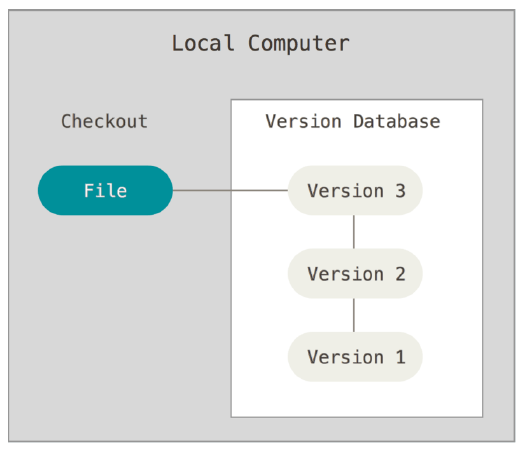
\includegraphics[scale=0.4]{LVC}  
	\caption[Local Version Control]{Local Version Control}
	\label{fig:LVC} 
\end{figure}

\subsubsection{Centralized Version Control System}
Dengan menggunakan Local Version Control System adalah bila ada beberapa orang yang berkolaborasi dengan developer. Karena pada Local Version Control System, version control dimiliki oleh masing-masing komputer sehingga pengguna tidak tahu apakah file tersebut sudah diubah oleh kolaborator lain. CVCS(Centralized Version Control System) memiliki sebuah server yang menyimpan semua file beserta historynya dan jumlah client yang mengecek file tersebut. Dengan adanya CVCS, semua orang mengetahui apa yang dilakukan oleh kolaborator yang mengerjakan pyoyek. Tetapi kelemahanya adalah ketika server tersebut down, tidak akan ada yang bisa berkolaborasi dan menyimpan perubahan yang sudah dikerjakan. Selain itu apabila data di server tersebut hilang maka dan tidak melakukan back-up, proyek yang sedang dikerjakan akan hilang beserta semua historinya. Struktur CVCS dapat dilihat pada Gambar~\ref{fig:CVCS}.

\begin{figure}[H]
	\centering  
	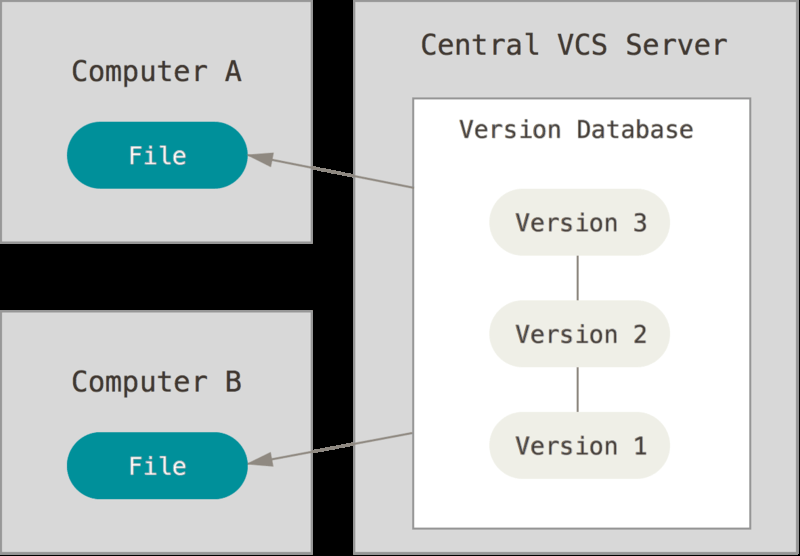
\includegraphics[scale=0.4]{CVCS}  
	\caption[Centralized Version Control]{Centralized Version Control}
	\label{fig:CVCS} 
\end{figure}

\subsubsection{Distributed Version Control System}
Dalam DVCS(Distributed Version Control System) seperti Git, Mercurial, Bazaar dan Darcs, client tidak mengecek version terbaru dari file tetapi client menggandakan repository termasuk historinya. Jika server mati/kehilangan data, maka client memiliki back-up file untuk mengembalikanya.  Ilustrasi DVCS terdapat pada Gambar~\ref{fig:DVCS}.

\begin{figure}[H]
	\centering  
	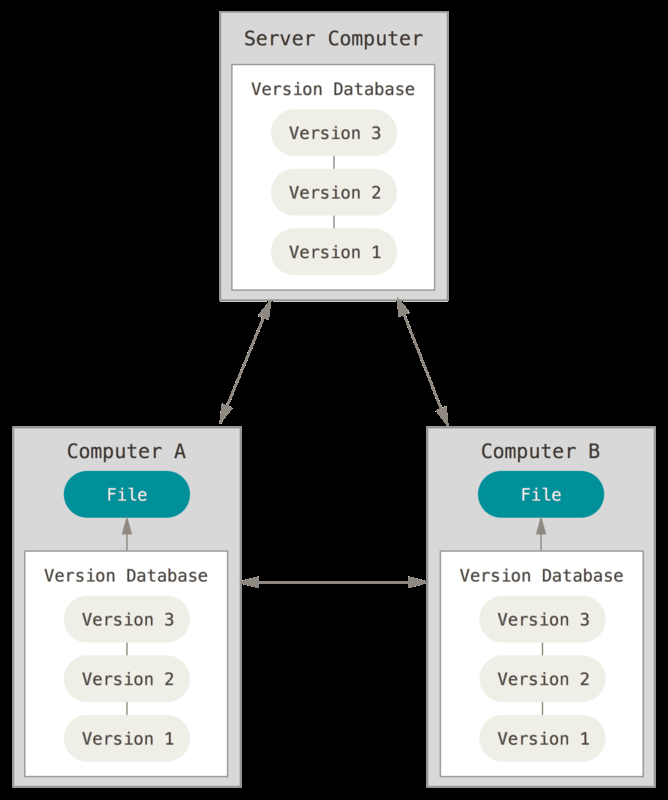
\includegraphics[scale=0.4]{DVCS}  
	\caption[Distributed Version Control]{Distributed Version Control}
	\label{fig:DVCS} 
\end{figure}

\subsection{Git}
Git merupakan sebuah version control namun berbeda dengan VCS lainnya dilihat dari cara menyimpan datanya. Sistem seperti CVS, Subversion, Perforce, Bazzar menyimpan data sebagai sekumpulan file dan perubahan setiap file disimpan setiap waktu. Pada Git, data tersebut dianggap sebagain sekumpulan snapshot dari miiature filesystem. Setiap commit atau menyimpan proyek, Git seolah-olah mengambil gambar untuk melihat seperti apa file yang terlihat pada saat itu dan menyimpannya sebagai referensi pada snapshot tersebut. Singkatnya, apabila tidak ada file yang diubah, Git tidak akan menyimpan file lagi.\\

Hampir semua operasi pada Git dapat dilakukan secara lokal. Ketika ingin menlihat histori suatu proyek, Git akan mengambil data histori tersebut dari basis data lokal, sehingga tidak perlu memintanya ke server. Selain itu, pengguna dapat bekerja secara offline. Pada sistem lain seperti Perforce, pengguna tidak dapat melakukan banyak hal jika tidak terkoneksi ke server dan pada CVS, pengguna dapat mengedit file tetapi tidak dapat commit ke basis data. Pada Git, pengguna dapat commit dikarenakan Git memiliki basis data lokal.\\

Git memiliki 3 state utama pada file yaitu: 

\begin{itemize}
	\item committed : data sudah tersimpan di basis data lokal.
	\item modified : file sudah diubah namun belum dicommit ke basis data.
	\item staged : menandai file yang sudah dimodifikasi dalam versi sekarang untuk dicommit.
\end{itemize}

Terdapat 3 bagian utama dalam proyek Git yaitu : 

\begin{itemize}
	\item Git directory : tempat untuk menyimpan metadata dan objek basis data untuk proyek yang dibuat. Ini adalah bagian terpenting dari Git dan inilah yang di-copy ketika clone repository dari komputer lain.
	\item Working tree : single checkout sebuah versi dari proyek. File diambil dari basis data yang sudah dicompressed di Git directory dan disimpan pada disk untuk digunakan dan dimodifikasi.
	\item Staging area : sebuah file yang ada di Git directory yang menyimpan informasi tentang apa yang akan disimpan untuk commit selanjutnya.  
\end{itemize}

Gambar~\ref{fig:gitState} di bawah ini menunjukan working tree, staging area dan Git directory.

\begin{figure}[H]
	\centering  
	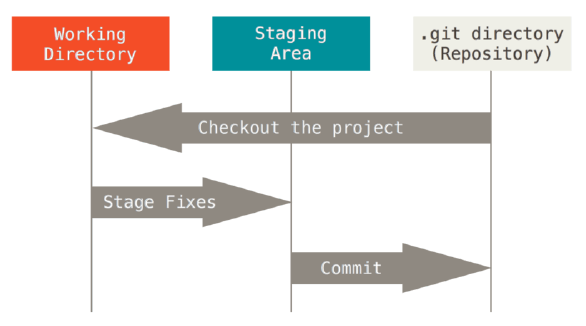
\includegraphics[scale=0.4]{gitState}  
	\caption[Working tree, staging area, dan Git directory]{Working tree, staging area, dan Git directory}
	\label{fig:gitState} 
\end{figure}

Workflow pada Git adalah sebagai berikut :

\begin{enumerate}
	\item Pengguna memodifikasi file di working tree milik pengguna.
	\item Pengguna memilih file yang akan menjadi bagian dari commit selanjutnya. File yang dipilih tersebut akan ditambahkan ke staging area. 
	\item Pengguna commit file tersebut yang berada pada staging area dan menyimpan snapshot secara permanen ke Git directory.
\end{enumerate}

Apabila versi tertentu dari sebuah file sudah ada pada Git directory, maka file tersebut dalam state committed. Jika file sudah dimodifikasi dan sudah ditambahkan ke staging area, maka file tersebut dalam state stage. Jika file sudah diubah dan sudah dicheckout tetapi belum dalam state staged, maka file tersebut dalam state modified.


\subsection{Git Branching}

\subsection{GitHub}
GitHub merupakan single host terbesar untuk Git repository dan sebagai titik tengah dari kolaborasi untuk jutaan pengembang dan proyek. Persentase terbesar dari semua Git repository dihosting di GitHub dan banyak proyek open-source menggunakanya untuk Git hosting, code review, issue tracking dan lainnya. 

\subsubsection{Fork}
Jika pengguna ingin berkontribusi pada proyek yang sudah ada dan pengguna tidak memiliki akses untuk push, maka pengguna dapat fork proyek tersebut. Ketika proyek tersebut telah di-fork, GitHub akan membuatkan sebuah copy/clone dari proyek tersebut yang sekarang sudah menjadi milik penggunanya dan dapat di-push. Orang lain dapat fork proyek, push proyek, dan berkontribusi dalam perubahan tersebut kembali ke repository aslinya dengan membuat Pull Request.\\

Untuk fork proyek, kunjungi halaman proyek dan klik tombol 'Fork' seperti pada Gambar~\ref{fig:forkButton} yang berada di atas kanan halaman. 

\begin{figure}[H]
	\centering  
	
\includegraphics[scale=1]{forkButton}  
	\caption[Tombol 'Fork']{Tombol 'Fork'}
	\label{fig:forkButton} 
\end{figure}

Github didesain untuk collaboration workflow tertentu yang berfokus pada Pull Request. Flow ini akan bekerja bila pengguna berkolaborasi dengan perusahhan yang globally-distributed atau beberapa orang asing berkontribusi dalam sebuah proyek melalui banyak fork. Flownya adalah sebagai berikut :

\begin{enumerate}
	\item Fork proyek.
	\item Buat topic branch dari master.
	\item Lakukan beberapa commit untuk memperbaiki proyek.
	\item Push branch ini ke proyek GitHub.
	\item Buka Pull Request di GitHub.
	\item Diskusikan dan commit.
	\item Pemilik proyek merges/menggabungkan atau menutup Pull Requset.
\end{enumerate}

\subsubsection{Pull Request}
Pull Request membuka tempat diskusi dengan code review dan owner(pemilik repository) dan kontributor dapat berkomunikasi tentang perubahan tersebut sampai owner merasa puas dan senang. Setelah itu owner akan merge/menggabungkan perubahan tersebut. Untuk membuat Pull Request, bukalah halaman 'Branches' dan buat Pull Request baru dari halaman tersebut dengan menklik tombol hijau seperti pada Gambar.... Sesudah mengklik tombol untuk membuat Pull Request baru, akan muncul sebuah laman yang meminta mengisi judul Pull Request dan deskripsi seperti pada Gambar.... Ketika tombol 'Create pull request' diklik,  maka pemilik proyek akan mendapatkan notifikasi bahwa seseorang menyarankan sebuah perubahan dan akan menghubungkan ke sebuah halaman yang memiliki semua informasi tersebut.

